\documentclass[tikz,border=1cm]{standalone}
\usetikzlibrary{arrows.meta,positioning,shapes.geometric,calc}
\tikzset{
  base/.style={%
    draw,align=center,
    minimum width=2.2cm,
    minimum height=0.9cm,
  },
  state/.style 2 args={%
    base,
    label={[inner sep=1.5pt, anchor=south west]north west:#1},
    label={[font=\ttfamily, inner sep=1.5pt, anchor=south east]north east:#2},
  },
  decision/.style={%
    base,diamond,
    aspect=2.444,
    inner sep=0pt
  },
  conditional/.style={%
    trapezium,base,
    trapezium stretches=true,
    shape aspect=2.444,
    trapezium left angle=70,
    trapezium right angle=110,
    inner xsep=0pt,inner ysep=2pt,
    anchor=center,fill=white,
    minimum height=0.35cm,
    minimum width=1.2cm,
  },
  pinlabel/.style={%
    inner ysep=0pt,
    label={[font=\sffamily,fill=white,inner sep=1pt,inner ysep=0pt]above:#1}
  }
}

\begin{document}
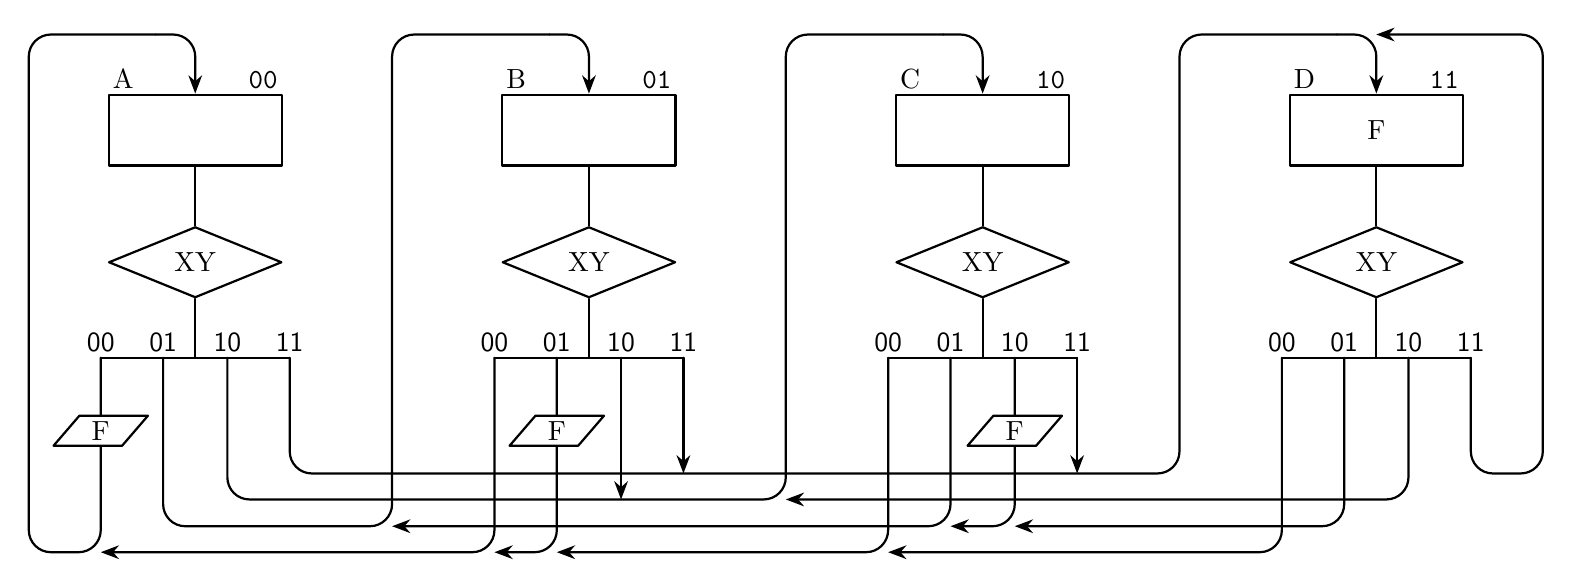
\begin{tikzpicture}[
    node distance=0.75cm,
    auto,thick,>=Stealth,
    line cap=round,line join=round,
    pics/mypic/.style n args={3}{%
        code = {%
            \node[draw,decision] (diamond) {XY};
            \node[above=of diamond,state={#2}{#3}] (rect) {#1};
            \draw[<-,rounded corners=8pt] (rect.north) |- ++(-.5cm,.75cm) coordinate (-up);
            \coordinate (tmp) at ([yshift=-.75cm]diamond.south);
            \draw[thick]  ([xshift=-1.2cm]tmp) --                     
            node[pos=0,pinlabel={00}] (-a) {} 
            node[pos=.33,pinlabel={01}] (-b) {} 
            node[pos=.67,pinlabel={10}] (-c) {} 
            node[pos=1,pinlabel={11}] (-d) {} 
            ([xshift=1.2cm]tmp);
            \path[thick] 
                (diamond.north) edge (rect.south)
                (tmp) edge (diamond.south)
            ;
        }
    }
]
\pic at (-7.5,0) (X) {mypic={}{A}{00}};
\pic at (-2.5,0) (Y) {mypic={}{B}{01}};
\pic at (2.5,0) (Z) {mypic={}{C}{10}};
\pic at (7.5,0) (W) {mypic={F}{D}{11}};
\coordinate (y1) at ([yshift=-1.5cm]X-a);
\coordinate (y2) at ([yshift=-1.83cm]X-a);
\coordinate (y3) at ([yshift=-2.17cm]X-a);
\coordinate (y4) at ([yshift=-2.5cm]X-a);
\coordinate (x1) at ([xshift=-1cm]Xrect.west);
\coordinate (x2) at ($(Xrect.east)!0.5!(Yrect.west)$);
\coordinate (x3) at ($(Yrect.east)!0.5!(Zrect.west)$);
\coordinate (x4) at ($(Zrect.east)!0.5!(Wrect.west)$);
\coordinate (x5) at ([xshift=1cm]Wrect.east);
% \draw[dashed,magenta]
% (x1) -- ++(0,-5)
% (x2) -- ++(0,-5)
% (x3) -- ++(0,-5)
% (x4) -- ++(0,-5)
% (x5) -- ++(0,-5)
% (y1) -- ++(25,0)
% (y2) -- ++(25,0)
% (y3) -- ++(25,0)
% (y4) -- ++(25,0)
% ;
\begin{scope}[rounded corners=8pt]
    % X node
    \draw (X-b) |- (y3-|x2) |- (Y-up);
    \draw (X-c) |- (y2-|x3) |- (Z-up);
    \draw (X-d) |- (y1-|x4) |- (W-up);
    \draw (X-a) -- node[pos=0.375,conditional,rounded corners=0pt] {F} (y4-|X-a) -- (y4-|x1) |- (X-up);
    % Y node
    \draw[->] (Y-a) |- (y4-|X-a);
    \draw[->] (Y-b) -- node[pos=0.375,conditional,rounded corners=0pt] {F} (y4-|Y-b) -- (y4-|Y-a);
    \draw[->] (Y-c) -- (y2-|Y-c);
    \draw[->] (Y-d) -- (y1-|Y-d);
    % Z node
    \draw[->] (Z-a) |- (y4-|Y-b);
    \draw[->] (Z-b) |- (y3-|x2);
    \draw[->] (Z-c) |- (y3-|Z-b);
    \draw[draw=none] (Z-c) -- node[pos=0.375,conditional,rounded corners=0pt] {F} (y4-|Z-c); % only located
    \draw[->] (Z-d) -- (y1-|Z-d);
    % W node
    \draw[->] (W-a) |- (y4-|Z-a);
    \draw[->] (W-b) |- (y3-|Z-c);
    \draw[->] (W-c) |- (y2-|x3);
    \draw[->] (W-d) |- (y1-|x5) |- ([xshift=.5cm]W-up);
\end{scope}
\end{tikzpicture}
\end{document}